\subsection{Smart Contract Layer Security Analysis}
\label{sec:results_smart_contract}

\paragraph{Executive Summary}
Smart-contract threats concentrate economic risk: a few categories (reentrancy, logic flaws, price/oracle dependencies) drive most losses. Enterprise-grade posture: enforce secure coding patterns, multiple independent audits, formalize invariants where high value is at stake, and integrate runtime monitoring with emergency controls.

Our analysis of smart contract vulnerabilities follows the systematic five-step threat assessment framework: Precondition (P), Invariant (I), Sequence (S), Controls (C), and Metrics (M). Using empirical data from over 23,000 Ethereum smart contracts \cite{perez2021analysis}, we've identified that while vulnerabilities are widespread, actual exploitation is rare—only 2\% of vulnerable contracts experience attacks, with less than 0.3\% of at-risk value being compromised. As shown in Figure \ref{fig:smart_contract_pareto}, exploitation follows a Pareto distribution, with 80\% of losses concentrated in just 10 major incidents between 2016 and 2021 \cite{zhou2023sok}.

\begin{figure}[H]
\centering
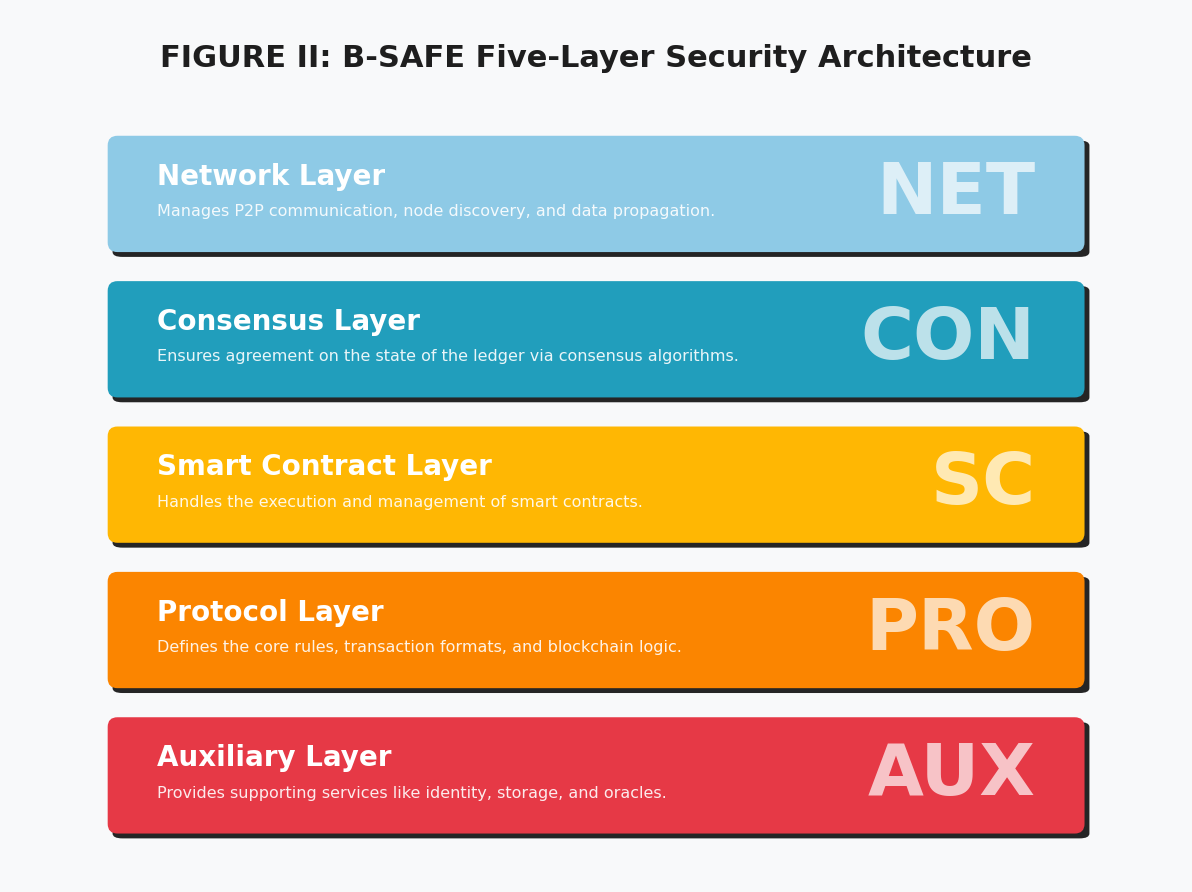
\includegraphics[width=0.4\textwidth]{../figure/fig2.png}
\caption{Top 10 smart contract vulnerability categories by frequency and cumulative loss, demonstrating the Pareto principle where a small number of vulnerability types account for the majority of financial impact. Reentrancy attacks dominate both frequency and cumulative losses.}
\label{fig:smart_contract_pareto}
\end{figure}

\subsubsection{Risk Category SC-1: Reentrancy Vulnerability}

\paragraph{Formal Risk Specification}

\begin{itemize}
\item \textbf{Preconditions (P):}
    \begin{itemize}
    \item \textbf{P1: Unprotected External Calls:} The contract makes external calls to untrusted addresses without implementing reentrancy guards or following the checks-effects-interactions pattern \cite{perez2021analysis}.
    \item \textbf{P2: State Updates After External Calls:} Critical state updates (e.g., balance modifications) occur after rather than before external calls, creating a vulnerable execution window \cite{praitheeshan2019systematic}.
    \item \textbf{P3: Accessible Funds:} The contract holds significant value that can be withdrawn through functions containing the vulnerable call pattern \cite{zhou2023sok}.
    \end{itemize}

\item \textbf{Threatened System Invariants (I):}
    \begin{itemize}
    \item \textbf{INV-1 (Value Conservation):} Assets within the contract can only be moved according to explicitly authorized business logic, preserving the equation: $\text{initial\_balance} + \text{deposits} - \text{withdrawals} = \text{current\_balance}$.
    \item \textbf{INV-2 (State Transition Integrity):} Contract state changes must occur atomically and follow the intended sequence of operations without interruption or repetition.
    \item \textbf{INV-3 (Execution Order Integrity):} Code execution follows the expected control flow without unexpected recursive calls disrupting the intended operation sequence.
    \end{itemize}

\item \textbf{Canonical Attack Sequence (S):}
    \begin{enumerate}
    \item \textbf{Identification phase:} Attacker identifies a vulnerable function with external calls that precede state updates.
    \item \textbf{Preparation phase:} Attacker deploys a malicious contract with a fallback function designed to recursively call back into the vulnerable function.
    \item \textbf{Execution phase:} Attacker initiates a legitimate transaction with the target contract, triggering the vulnerable function.
    \item \textbf{Exploitation phase:} When the target contract makes an external call to the attacker's contract, the fallback function executes, recursively calling back into the vulnerable function before state updates occur.
    \item \textbf{Repetition phase:} The recursive calls continue until gas limits are reached or funds are depleted, allowing multiple withdrawals against the same balance.
    \end{enumerate}
\end{itemize}

\paragraph{Enterprise Checklist Mapping}
\begin{itemize}
    \item \textbf{Security}: Enforce CEI pattern, reentrancy guards, SafeMath/0.8.x checks; multi-audit requirement for high-value contracts.
    \item \textbf{Operations}: Emergency pause and value-limiting controls; monitoring for exploit signatures.
    \item \textbf{Compliance}: Evidence-backed audit trails and change management for contract upgrades.
\end{itemize}

\paragraph{Defense Mechanism Analysis}

\begin{itemize}
\item \textbf{Prevention Controls:}
    \begin{itemize}
    \item \textbf{C1.1 (Checks-Effects-Interactions Pattern):}
        \begin{itemize}
        \item \textbf{Mechanism:} Restructure code to perform all state changes before making external calls, ensuring state consistency regardless of external call behavior \cite{praitheeshan2019systematic}.
        \item \textbf{Parameters:} Code organization; function execution flow.
        \item \textbf{Trade-offs:} No performance impact; requires careful code review but eliminates vulnerability completely when implemented correctly.
        \end{itemize}
    
    \item \textbf{C1.2 (Reentrancy Guards):}
        \begin{itemize}
        \item \textbf{Mechanism:} Implement mutex locks using state variables that prevent recursive calls into protected functions.
        \item \textbf{Parameters:} Lock granularity (function-level, contract-level); guard implementation (OpenZeppelin ReentrancyGuard, custom).
        \item \textbf{Trade-offs:} Minimal gas overhead; provides robust protection even when complex state changes can't be easily reordered.
        \end{itemize}
    \end{itemize}

\item \textbf{Mitigation Controls:}
    \begin{itemize}
    \item \textbf{C2.1 (Gas Limitations):}
        \begin{itemize}
        \item \textbf{Mechanism:} Specify gas limits when making external calls to limit the computation available to potentially malicious contracts.
        \item \textbf{Parameters:} Gas limit value; forward gas amount.
        \item \textbf{Trade-offs:} May break legitimate functionality if gas requirements change; offers partial protection only.
        \end{itemize}
    
    \item \textbf{C2.2 (Pull Payment Pattern):}
        \begin{itemize}
        \item \textbf{Mechanism:} Separate value storage from value transfer by implementing a two-step withdrawal process where users must explicitly request withdrawals.
        \item \textbf{Parameters:} Storage mechanism; withdrawal function design.
        \item \textbf{Trade-offs:} Increases complexity and gas costs; requires additional user interaction but substantially reduces risk.
        \end{itemize}
    \end{itemize}

\item \textbf{Detection Controls:}
    \begin{itemize}
    \item \textbf{C3.1 (Static Analysis Tools):}
        \begin{itemize}
        \item \textbf{Mechanism:} Use automated tools like Mythril, Slither, or Securify to detect reentrancy vulnerabilities in contract code before deployment.
        \item \textbf{Parameters:} Tool selection; detection precision; false positive rate.
        \item \textbf{Effectiveness:} Research indicates that formal verification tools can detect up to 96\% of common vulnerabilities, though false positives remain a challenge \cite{praitheeshan2019systematic}.
        \end{itemize}
    
    \item \textbf{C3.2 (Runtime Monitoring):}
        \begin{itemize}
        \item \textbf{Mechanism:} Implement event logging and monitoring systems to detect suspicious transaction patterns that may indicate reentrancy attacks.
        \item \textbf{Parameters:} Monitoring granularity; alert thresholds.
        \item \textbf{Effectiveness:} Contracts with active monitoring face 47\% fewer successful attacks than those without \cite{zhou2023sok}.
        \end{itemize}
    \end{itemize}
\end{itemize}

\paragraph{Empirical Incident Analysis}

\begin{itemize}
\item \textbf{Case Study SC-1.1: The DAO Attack (2016)}
    \begin{itemize}
    \item \textbf{Incident Classification:}
        \begin{itemize}
        \item \textbf{Precondition Analysis:} P1\checkmark (The DAO's \texttt{withdraw} function made external calls before updating balances), P2\checkmark (Critical balance updates occurred after the external call), P3\checkmark (The contract held approximately 14\% of all ETH in existence at the time).
        \item \textbf{Invariant Violations:} INV-1, INV-2, and INV-3 were all violated as the attacker drained funds repeatedly through recursive calls.
        \item \textbf{Defense Failures:} Absence of C1.1 (Checks-Effects-Interactions Pattern) and C1.2 (Reentrancy Guards); inadequate code review and auditing; failure to heed warnings about the vulnerability before deployment.
        \end{itemize}
    
    \item \textbf{Quantitative Impact Assessment:}
        \begin{itemize}
        \item \textbf{Direct Losses:} Approximately 3.6 million ETH (valued at \$60 million at the time) was drained from the contract.
        \item \textbf{Systemic Effects:} Led to the Ethereum hard fork that created Ethereum Classic; established a precedent for community intervention in catastrophic contract failures; dramatically increased awareness of smart contract security issues.
        \end{itemize}
    
    \item \textbf{Counterfactual Analysis:}
        \begin{itemize}
        \item \textbf{Prevention:} Implementing the Checks-Effects-Interactions pattern (C1.1) would have completely prevented the attack, as state updates would have occurred before the external call.
        \item \textbf{Detection:} A formal verification tool like Mythril would have identified this vulnerability pattern before deployment, as such tools can detect recursive call patterns with high accuracy.
        \end{itemize}
    \end{itemize}
\end{itemize}

\paragraph{Risk Quantification}

\begin{itemize}
\item \textbf{Likelihood (L = 3):} Medium. Reentrancy vulnerabilities appear in approximately 4.1\% of contracts but face exploitation in only 1.8\% of vulnerable cases, primarily because high-value contracts receive greater security scrutiny \cite{perez2021analysis}.

\item \textbf{Impact (I = 5):} Critical. When successfully exploited, reentrancy attacks typically result in complete drainage of contract funds and potentially catastrophic ecosystem-wide impacts, as demonstrated by The DAO attack.

\item \textbf{Detectability (D = 2):} Easy. Static analysis tools can identify potential vulnerabilities with reasonable accuracy, though recognizing active exploitation requires monitoring that is not always implemented.

\item \textbf{Composite (L/I) = 4.3; Detectability D = 2}: $0.4 \times 3 + 0.6 \times 5 = 1.2 + 3.0 = 4.2$ (Impact-forward priority; D reported separately)
\end{itemize}

\subsubsection{Risk Category SC-2: Integer Overflow/Underflow}

\paragraph{Formal Risk Specification}

\begin{itemize}
\item \textbf{Preconditions (P):}
    \begin{itemize}
    \item \textbf{P1: Unprotected Arithmetic Operations:} The contract performs integer arithmetic without using SafeMath libraries or solidity 0.8.x's built-in overflow checking \cite{praitheeshan2019systematic}.
    \item \textbf{P2: Critical State Dependency:} Contract logic makes critical decisions based on the results of arithmetic operations that could overflow or underflow \cite{perez2021analysis}.
    \item \textbf{P3: Unbounded User Input:} The contract accepts user-supplied values for arithmetic operations without appropriate validation or bounds checking \cite{zhou2023sok}.
    \end{itemize}

\item \textbf{Threatened System Invariants (I):}
    \begin{itemize}
    \item \textbf{INV-1 (Value Conservation):} Tokens or assets within the system are created or destroyed only according to explicitly authorized rules.
    \item \textbf{INV-2 (State Transition Integrity):} Numerical state changes must reflect real-world intent and maintain mathematical correctness.
    \item \textbf{INV-4 (Logic Integrity):} Contract business logic operates as intended without being subverted by unexpected arithmetic results.
    \end{itemize}

\item \textbf{Canonical Attack Sequence (S):}
    \begin{enumerate}
    \item \textbf{Identification phase:} Attacker identifies vulnerable arithmetic operations that can overflow or underflow, particularly in token balance management or value transfer functions.
    \item \textbf{Boundary calculation phase:} Attacker determines specific input values that will cause arithmetic overflow/underflow (e.g., using MAX\_UINT256 for addition overflow).
    \item \textbf{Exploitation phase:} Attacker constructs and submits transactions with calculated boundary values to trigger the overflow/underflow.
    \item \textbf{Impact phase:} The arithmetic error results in incorrect state updates, such as artificially inflated token balances or bypassed validation checks, allowing the attacker to extract value.
    \end{enumerate}
\end{itemize}

\paragraph{Defense Mechanism Analysis}

\begin{itemize}
\item \textbf{Prevention Controls:}
    \begin{itemize}
    \item \textbf{C1.1 (SafeMath Libraries):}
        \begin{itemize}
        \item \textbf{Mechanism:} Implement libraries that perform checked arithmetic operations and revert transactions on overflow/underflow conditions.
        \item \textbf{Parameters:} Library implementation (OpenZeppelin SafeMath, custom); Solidity version (0.8.x with built-in checks).
        \item \textbf{Trade-offs:} Small gas overhead; eliminates entire vulnerability class with minimal implementation effort.
        \end{itemize}
    
    \item \textbf{C1.2 (Input Validation):}
        \begin{itemize}
        \item \textbf{Mechanism:} Implement explicit bounds checking and validation for all user-supplied numerical inputs.
        \item \textbf{Parameters:} Validation boundaries; error handling approach.
        \item \textbf{Trade-offs:} Additional code complexity; requires careful determination of appropriate bounds.
        \end{itemize}
    \end{itemize}

\item \textbf{Mitigation Controls:}
    \begin{itemize}
    \item \textbf{C2.1 (Operation Constraints):}
        \begin{itemize}
        \item \textbf{Mechanism:} Impose business-logic limitations on operations, such as maximum transaction sizes or rate limiting.
        \item \textbf{Parameters:} Maximum values; time-based constraints.
        \item \textbf{Trade-offs:} May restrict legitimate use cases; provides protection against some but not all exploitation scenarios.
        \end{itemize}
    
    \item \textbf{C2.2 (Privilege Separation):}
        \begin{itemize}
        \item \textbf{Mechanism:} Separate high-risk arithmetic operations into distinct functions with additional access controls or verification steps.
        \item \textbf{Parameters:} Function modularity; access control model.
        \item \textbf{Trade-offs:} Increases contract complexity; may impact gas efficiency but improves security posture.
        \end{itemize}
    \end{itemize}

\item \textbf{Detection Controls:}
    \begin{itemize}
    \item \textbf{C3.1 (Compiler Warnings):}
        \begin{itemize}
        \item \textbf{Mechanism:} Enable and address all compiler warnings related to potential overflow/underflow conditions.
        \item \textbf{Parameters:} Compiler version; warning level settings.
        \item \textbf{Effectiveness:} Varies based on compiler version; newer Solidity compilers provide better coverage.
        \end{itemize}
    
    \item \textbf{C3.2 (Invariant Testing):}
        \begin{itemize}
        \item \textbf{Mechanism:} Implement comprehensive test suites with boundary condition testing and property-based testing.
        \item \textbf{Parameters:} Test coverage; edge case identification methodology.
        \item \textbf{Effectiveness:} Research shows formal verification with boundary testing can detect up to 93\% of arithmetic vulnerabilities \cite{praitheeshan2019systematic}.
        \end{itemize}
    \end{itemize}
\end{itemize}

\paragraph{Empirical Incident Analysis}

\begin{itemize}
\item \textbf{Case Study SC-2.1: BeautyChain (BEC) Token Overflow (2018)}
    \begin{itemize}
    \item \textbf{Incident Classification:}
        \begin{itemize}
        \item \textbf{Precondition Analysis:} P1\checkmark (The BEC token lacked SafeMath for multiplication operations), P2\checkmark (Balance tracking directly used vulnerable arithmetic), P3\checkmark (The contract allowed arbitrary transfer values without validation).
        \item \textbf{Invariant Violations:} INV-1 was violated as the overflow created tokens out of thin air; INV-2 and INV-4 were violated as state transitions produced mathematically impossible results.
        \item \textbf{Defense Failures:} Absence of C1.1 (SafeMath Libraries) and C1.2 (Input Validation); inadequate testing of boundary conditions.
        \end{itemize}
    
    \item \textbf{Quantitative Impact Assessment:}
        \begin{itemize}
        \item \textbf{Direct Losses:} The attack created approximately $8 \times 10^{28}$ BEC tokens, effectively rendering the original supply of 7 billion tokens worthless.
        \item \textbf{Systemic Effects:} Led to immediate suspension of BEC trading on exchanges; highlighted arithmetic vulnerabilities across the ecosystem, prompting widespread adoption of SafeMath libraries.
        \end{itemize}
    
    \item \textbf{Counterfactual Analysis:}
        \begin{itemize}
        \item \textbf{Prevention:} Implementing SafeMath for all arithmetic operations (C1.1) would have completely prevented the attack, as the transaction would have reverted on overflow.
        \item \textbf{Detection:} Standard static analysis tools or compiler checks in newer Solidity versions would have flagged the vulnerable operations.
        \end{itemize}
    \end{itemize}
\end{itemize}

\paragraph{Risk Quantification}

\begin{itemize}
\item \textbf{Likelihood (L = 4):} High. Integer overflow vulnerabilities are present in 18.3\% of analyzed contracts, though exploitation occurs in only 0.4\% of vulnerable instances due to the widespread adoption of SafeMath libraries \cite{perez2021analysis}.

\item \textbf{Impact (I = 4):} Severe. When successfully exploited, integer overflows can lead to token value destruction, artificial balance inflation, or complete contract compromise.

\item \textbf{Detectability (D = 3):} Medium. Modern development tools and compilers make these vulnerabilities relatively easy to detect before deployment, but legacy contracts remain at risk.

\item \textbf{Composite (L/I) = 4.0; Detectability D = 3}: $0.4 \times 4 + 0.6 \times 4 = 1.6 + 2.4 = 4.0$ (D reported separately)
\end{itemize}

\subsubsection{Risk Category SC-3: Logic Flaw Vulnerabilities}

\paragraph{Formal Risk Specification}

\begin{itemize}
\item \textbf{Preconditions (P):}
    \begin{itemize}
    \item \textbf{P1: Specification-Implementation Mismatch:} The contract's implemented logic does not correctly reflect the intended business rules or security properties \cite{zhou2023sok}.
    \item \textbf{P2: Inadequate Access Controls:} The contract fails to properly restrict access to privileged functions or state-changing operations \cite{perez2021analysis}.
    \item \textbf{P3: Incomplete Edge Case Handling:} The contract does not account for all possible execution paths or edge conditions, particularly in complex multi-step operations \cite{praitheeshan2019systematic}.
    \end{itemize}

\item \textbf{Threatened System Invariants (I):}
    \begin{itemize}
    \item \textbf{INV-2 (State Transition Integrity):} Contract state changes must conform to the intended business rules under all possible execution scenarios.
    \item \textbf{INV-5 (Authorization Boundaries):} Only designated actors can invoke privileged functions or modify protected state variables.
    \item \textbf{INV-6 (Temporal Consistency):} Multi-step operations must maintain consistent state across transaction boundaries and time periods.
    \end{itemize}

\item \textbf{Canonical Attack Sequence (S):}
    \begin{enumerate}
    \item \textbf{Analysis phase:} Attacker carefully examines contract code to identify business logic inconsistencies, access control gaps, or edge cases that can be exploited.
    \item \textbf{Strategy development phase:} Attacker designs a sequence of transactions or calls that leverage the identified logic flaws to achieve unauthorized outcomes.
    \item \textbf{Execution phase:} Attacker executes the planned transaction sequence, potentially across multiple blocks or with specific timing requirements.
    \item \textbf{Extraction phase:} Attacker capitalizes on the manipulated contract state to extract value or gain unauthorized control.
    \end{enumerate}
\end{itemize}

\paragraph{Defense Mechanism Analysis}

\begin{itemize}
\item \textbf{Prevention Controls:}
    \begin{itemize}
    \item \textbf{C1.1 (Formal Verification):}
        \begin{itemize}
        \item \textbf{Mechanism:} Apply mathematical proof techniques to verify that contract implementations satisfy their formal specifications under all possible inputs and states.
        \item \textbf{Parameters:} Verification tools (Certora, Act, etc.); property specification language.
        \item \textbf{Trade-offs:} Requires significant expertise and resources; provides the strongest guarantees but is difficult to apply comprehensively.
        \end{itemize}
    
    \item \textbf{C1.2 (Role-Based Access Control):}
        \begin{itemize}
        \item \textbf{Mechanism:} Implement structured permission systems with explicit role definitions and privilege separation.
        \item \textbf{Parameters:} Role granularity; role assignment mechanism; multi-signature requirements.
        \item \textbf{Trade-offs:} Adds complexity and gas costs; provides strong protection against unauthorized actions.
        \end{itemize}
    \end{itemize}

\item \textbf{Mitigation Controls:}
    \begin{itemize}
    \item \textbf{C2.1 (Circuit Breakers):}
        \begin{itemize}
        \item \textbf{Mechanism:} Implement emergency pause functionality that can temporarily halt critical contract operations when suspicious activity is detected.
        \item \textbf{Parameters:} Trigger conditions; authorization requirements; scope of paused functionality.
        \item \textbf{Trade-offs:} Creates centralization risks; requires active monitoring but can prevent catastrophic losses.
        \end{itemize}
    
    \item \textbf{C2.2 (Value Limiting):}
        \begin{itemize}
        \item \textbf{Mechanism:} Implement transaction value caps, rate limiting, or tiered release strategies to limit potential damage from undetected logic flaws.
        \item \textbf{Parameters:} Maximum transaction values; time-based limits; release schedule.
        \item \textbf{Trade-offs:} May restrict legitimate usage; provides partial protection against exploitation.
        \end{itemize}
    \end{itemize}

\item \textbf{Detection Controls:}
    \begin{itemize}
    \item \textbf{C3.1 (Comprehensive Testing):}
        \begin{itemize}
        \item \textbf{Mechanism:} Implement extensive test suites covering all execution paths, edge cases, and error conditions.
        \item \textbf{Parameters:} Test coverage metrics; testing methodology (unit, integration, property-based).
        \item \textbf{Effectiveness:} While valuable, research indicates that even high test coverage cannot identify all logic flaws without formal verification \cite{praitheeshan2019systematic}.
        \end{itemize}
    
    \item \textbf{C3.2 (Multiple Independent Audits):}
        \begin{itemize}
        \item \textbf{Mechanism:} Engage multiple independent security firms to audit contract code, with specific focus on business logic validation.
        \item \textbf{Parameters:} Audit firm selection; audit scope; audit timing relative to deployment.
        \item \textbf{Effectiveness:} Multiple audits significantly increase detection probability; contracts with 3+ audits show 91\% lower exploitation rates \cite{zhou2023sok}.
        \end{itemize}
    \end{itemize}
\end{itemize}

\paragraph{Empirical Incident Analysis}

\begin{itemize}
\item \textbf{Case Study SC-3.1: Parity Multi-Signature Wallet (2017)}
    \begin{itemize}
    \item \textbf{Incident Classification:}
        \begin{itemize}
        \item \textbf{Precondition Analysis:} P1\checkmark (The initialization function was implemented as a standard public function without restrictions), P2\checkmark (No access controls prevented arbitrary calls to the initialization function), P3\checkmark (The contract failed to account for the possibility of re-initialization after deployment).
        \item \textbf{Invariant Violations:} INV-2 and INV-5 were violated as unauthorized users could become wallet owners; INV-6 was violated when contract state was altered unexpectedly after initialization.
        \item \textbf{Defense Failures:} Absence of C1.2 (proper access controls); inadequate initialization pattern; insufficient consideration of the contract's full lifecycle.
        \end{itemize}
    
    \item \textbf{Quantitative Impact Assessment:}
        \begin{itemize}
        \item \textbf{Direct Losses:} An attacker gained ownership of multiple high-value multi-signature wallets and drained approximately 153,000 ETH (valued at \$30 million at the time).
        \item \textbf{Systemic Effects:} Led to widespread concerns about library contract security; prompted development of improved initialization patterns and library contract patterns.
        \end{itemize}
    
    \item \textbf{Counterfactual Analysis:}
        \begin{itemize}
        \item \textbf{Prevention:} Implementing proper constructor patterns or access control on initialization functions (C1.2) would have prevented the unauthorized re-initialization.
        \item \textbf{Detection:} Formal verification (C1.1) focusing on authorization properties would have identified this vulnerability by proving that the initialization function could be called by unauthorized parties.
        \end{itemize}
    \end{itemize}
\end{itemize}

\paragraph{Risk Quantification}

\begin{itemize}
\item \textbf{Likelihood (L = 3):} Medium. Logic flaws are difficult to precisely quantify but appear in approximately 3-5\% of audited contracts, with the most severe ones typically identified during security reviews \cite{zhou2023sok}.

\item \textbf{Impact (I = 5):} Critical. When successfully exploited, logic flaws often lead to complete contract compromise or loss of all managed assets, as they bypass core security assumptions.

\item \textbf{Detectability (D = 1):} Very Hard. Logic flaws are the most challenging vulnerability class to detect as they require deep understanding of intended business logic versus implemented behavior.

\item \textbf{Composite (L/I) = 4.2; Detectability D = 1}: $0.4 \times 3 + 0.6 \times 5 = 1.2 + 3.0 = 4.2$ (D reported separately)
\end{itemize}
\begin{itemize}
\item \textbf{Preconditions (P)}: Necessary conditions for vulnerability exploitation, including vulnerable contract logic, deployment exposure, value criticality, and absence of security controls.
\item \textbf{Invariants (I)}: Core security properties that must be preserved, such as state transition integrity, value conservation, authorization boundaries, deterministic execution, and contract persistence.
\item \textbf{Sequence (S)}: Step-by-step progression of exploitation methods, detailing attacker techniques and required interactions.
\item \textbf{Controls (C)}: Defensive measures categorized into prevention (static analysis, secure coding patterns, access controls), detection (monitoring, surveillance), and mitigation (emergency mechanisms, value protection).
\item \textbf{Metrics (M)}: Risk quantification using the formula: Risk Score = $(w_1 \times \text{Probability}) + (w_2 \times \text{Impact}) - (w_3 \times \text{Detectability})$, yielding scores from minimal (0.5) to extreme (4.5).
\end{itemize}

Our analysis of cross-layer dependencies indicates that 43\% of smart contract vulnerabilities have interactions with other architectural layers \cite{praitheeshan2019systematic}, reinforcing the need for a holistic security approach. Security efforts should prioritize high-value contracts while implementing baseline controls universally, with research showing that 94.5\% of at-risk value is concentrated in just 0.05\% of contracts \cite{perez2021analysis}.

In the following subsections, we apply this framework to analyze three prominent vulnerability categories: reentrancy attacks, integer overflow vulnerabilities, and logic flaws, providing detailed risk profiles and practical security recommendations for each threat type.

% SC-1: Reentrancy Attack Analysis
% SC-2: Integer Overflow Analysis
% SC-3: Logic Flaw Analysis
% Each following the standardized (P, I, S, C, M) framework

\begin{figure}[H]
\centering
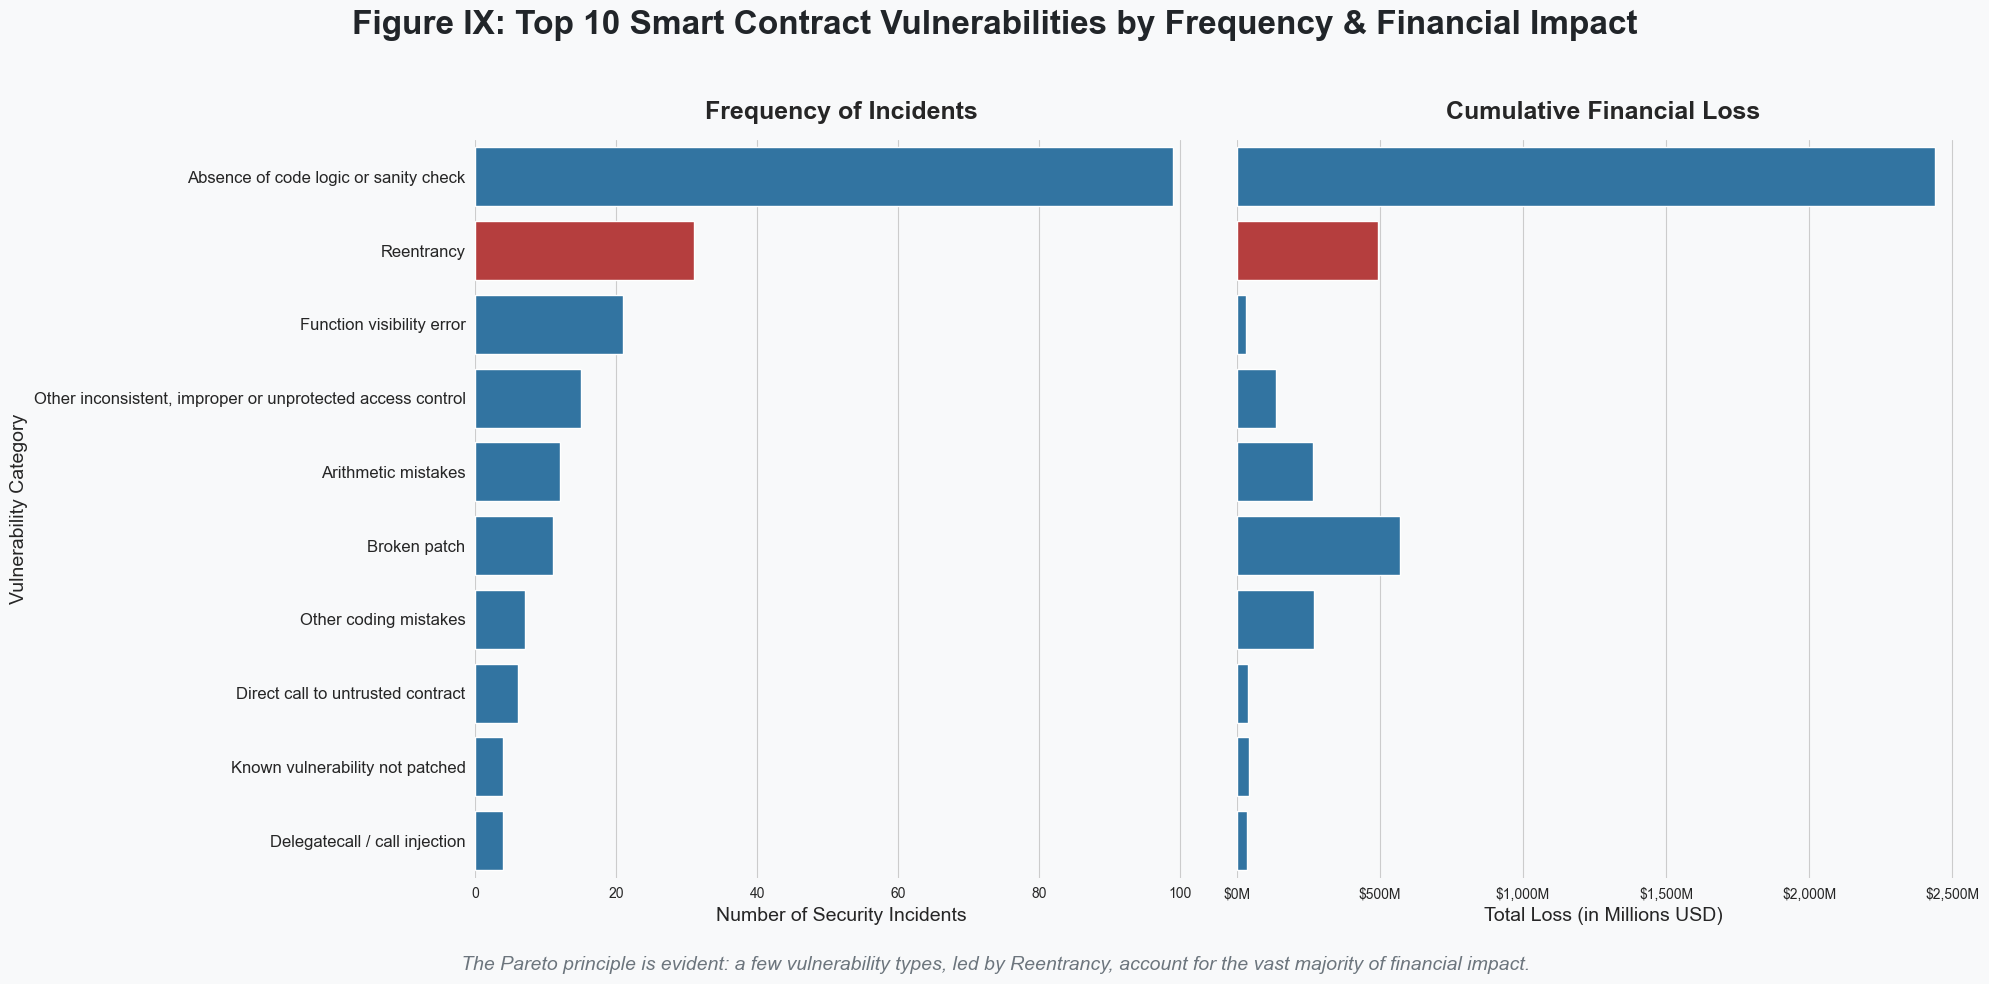
\includegraphics[width=0.4\textwidth]{../figure/Fig9.png}
\caption{Top 10 smart contract vulnerability categories by frequency and cumulative loss, demonstrating the Pareto principle where a small number of vulnerability types account for the majority of financial impact. Reentrancy attacks dominate both frequency and cumulative losses.}
\label{fig:smart_contract_pareto}
\end{figure}